\documentclass{standalone}
\usepackage{amsmath}
\usepackage[dvipsnames]{xcolor}
\usepackage{scalerel}
\usepackage{tikz} 
\usetikzlibrary{arrows, decorations.markings,decorations.pathreplacing,angles,quotes}
\usepackage{microtype}
\usepackage{fourier}

\definecolor{py_blue}{rgb}{0.12156862745098039, 0.4666666666666667, 0.7058823529411765}
\definecolor{py_orange}{rgb}{1.0, 0.4980392156862745, 0.054901960784313725}
\definecolor{py_green}{rgb}{0.17254901960784313, 0.6274509803921569, 0.17254901960784313}
\definecolor{py_red}{rgb}{0.8392156862745098, 0.15294117647058825, 0.1568627450980392}
\definecolor{py_purple}{rgb}{0.5803921568627451, 0.403921568627451, 0.7411764705882353}

\begin{document}

\begin{tikzpicture}
	\node[anchor=south west,inner sep=0] (Bild) at (0,0) {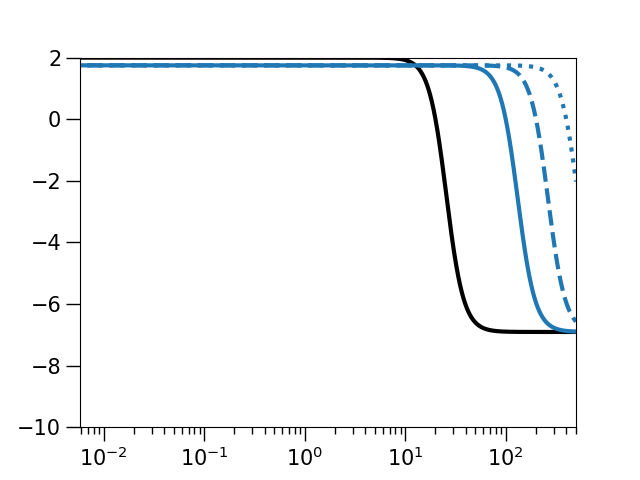
\includegraphics[scale=0.39]{hypo1_blank}};
   		\begin{scope}[x=(Bild.south east),y=(Bild.north west)]
        	\draw (0.5,-0.035) node {\small antibiotic concentration $c$};
        	\draw (-0.09,0.5) node [rotate=90] {\small bacterial net growth rate};
        	\draw (-0.02,0.5) node [rotate=90] {\small $\beta_j-\delta_j-\alpha_j(c)$};
        	
			\draw[thick,color=black] (0.14,0.44) -- node[right=5pt] {\tiny \color{black} $\alpha_{\scaleto{S}{2.5pt}}(c)$, $\text{mic}_{\scaleto{S}{2.5pt}}=0.017$} (0.19,0.44);        	
			\draw[thick,color=py_blue] (0.14,0.36) -- node[right=5pt] {\tiny \color{black} $\alpha_{\scaleto{R}{2.5pt}}(c)$, $\text{mic}_{\scaleto{R}{2.5pt}}=5\times\text{mic}_{\scaleto{S}{2.5pt}}$} (0.19,0.36);     
			\draw[thick,color=py_blue,dashed] (0.14,0.28) -- node[right=5pt] {\tiny \color{black} $\alpha_{\scaleto{R}{2.5pt}}(c)$, $\text{mic}_{\scaleto{R}{2.5pt}}=10\times\text{mic}_{\scaleto{S}{2.5pt}}$} (0.19,0.28);  
			\draw[thick,color=py_blue,dotted] (0.14,0.2) -- node[right=5pt] {\tiny \color{black} $\alpha_{\scaleto{R}{2.5pt}}(c)$, $\text{mic}_{\scaleto{R}{2.5pt}}=20\times\text{mic}_{\scaleto{S}{2.5pt}}$} (0.19,0.2);      
			
    	\end{scope}
\end{tikzpicture}

\end{document}